% !TeX spellcheck = en_US
% !TeX encoding = UTF-8
% !TeX root = ../document.tex

\newcommand{\lumiA}{\SI{2.3}{\per\femto\barn}}
\newcommand{\lumiB}{\SI{35.9}{\per\femto\barn}}

\chapter{Discovery Potential}
\label{chap:sensitivity_studies}

The study of the discovery potential, also called \emph{sensitivity study}, has multiple purposes: On one hand, its goal is to assess the absolute sensitivity of the analysis towards certain benchmark models for new physics. But on the other hand, it can also be used to evaluate the sensitivity for a single model using different analysis variants. This allows us to assess which features, such as algorithms or parameters, have the largest impact on the discovery potential.

The chapter will start with the latter goal: After defining a set of features and key questions to be answered in this chapter, we will present the corresponding results in form of tables and graphics and move to a conclusion. 
In the second part, the sensitivity towards the benchmark models introduced earlier will be explicitly assessed and compared to dedicated analyses performed on a similar dataset by \ac{CMS}.

\subsubsection{Key Questions}
\begin{itemize}
    \item Validation: Using only the \ac{SM} as new physics input, are the \ptilde-distribution and \phat results inconclusive, as expected?
    \item How does the \ptilde distribution of the \ac{SM}-only scan scale with luminosity?
    \item How does the minimum-yield-per-event-class threshold (\fref{sec:min_yield}) affect the \ac{SM}-only distribution?
    \item How do the region vetoes (including the overcoverage veto introduced in \fref{sec:overcoverage_veto}) impact the available search space?
    \item Is \ac{MUSiC} sensitive to new physics that are only visible in one or few final states?
    \item Is \ac{MUSiC} sensitive to new physics that have a smaller impact on several final states?    
    \item Which test statistic for \phat shows the best sensitivity?
    %\item How does an increase in luminosity affect the sensitivity? For which kind of models does the analysis benefit from a higher luminosity?
    %\item How do \Pqb-tagged jets affect the sensitivity?
\end{itemize}

\subsection{Interpretation of the Result Plots}
\label{sec:how_to_read_plots}

The result figures presented in the following sections contain a large amount of information for readers not accustomed to \ac{MUSiC}. Therefore, this section aims to quickly introduce the material used to present the results and explain how they can be interpreted. An overview of the information presented is schematically shown in \fref{fig:results_flow}.

\begin{figure}
    \centering
    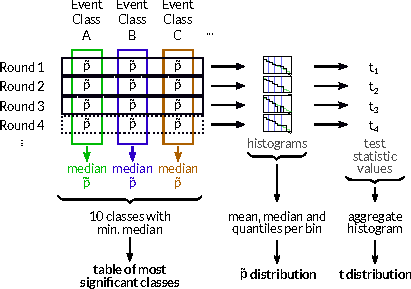
\includegraphics[width=0.7\textwidth]{ptilde_distrib_and_sign_classes}
    \caption{Flow of information from the sets of \ptilde values to the results presented in this chapter. The schematic shows the vertical aggregation of \ptilde values from $\nrounds = 4$ pseudo-experiments into median \ptilde values as well as the horizontal aggregation of distributions of \ptilde values for each round. Furthermore, the test statistic \TSphat is also computed horizontally and aggregated into a distribution.}
    \label{fig:results_flow}
\end{figure}

\subsubsection{\ptilde-Distribution}
This illustration has conceptually been introduced in \fref{sec:ptilde_distribution}. One example can be seen in \fref{fig:result_validation_ptilde}.
It is produced by aggregating $-\log_{10}{\ptilde}$ values: First, for each of the \nrounds rounds, the \nclasses results from \nclasses classes are sorted into a histogram. This results in \nrounds histograms, therefore \nrounds entries per bin. In each bin, the median bin content, the mean bin content and \SI{68}{\percent}- and \SI{95}{\percent} quantiles around the median are calculated. The highest bin serves as overflow bin, as we cannot obtain a precise value for $\ptilde < \num{1e-4}$ from \num{10000} \ac{SM}-only pseudo-experiments.

The aggregation procedure is done for the (corrected) \ptilde values originating from searches for deviations between the \ac{SM} and pseudo-experiments based on the \ac{SM} and its result is depicted in the turquoise and blue bands, as well as the turquoise line and the black dotted line. 
Additionally, the illustrations show a dashed green line which represents a uniform distribution. Because of the logarithmic binning, the number of uniform events is not equal for each bin. The uniform distribution can be used to tell whether \ptilde fulfills the requirement of a $p$-value of being uniformly distributed.

Results of the pseudo-experiments originating from a signal study (see \fref{sec:signal_study}) are depicted within the same figure as red data points. The vertical error bar around these points indicate the \SI{68}{\percent} quantiles around the median. This thesis uses \num{100} signal pseudo-experiments for each event class, thus \num{100} bin contents have been used to calculate the magnitude of the error bar.

\subsubsection{Table of Most Significant Classes}
The second result presentation is the table of most significant classes. It is aggregated by regarding the corrected \ptilde-values of each event class for all rounds. For each event class, the median \ptilde value is computed. Subsequently, the event classes with the \num{10} smallest medians are presented, alongside with the $Z$-score expressing the deviation in terms of standard deviations of a normal distribution (for the conversion formula, see \fref{app:z_score}). 

\subsubsection{Distributions of \TSphat}
The third way of presenting the results is by aggregating distributions of \TSphat values. Several examples are shown in \fref{fig:result_validation_phat}. There are always multiple distributions depicted in one figure: The distribution filled in gray shows the distribution of \TSphat values from \ac{SM}-pseudo-experiments. In addition there is at least one distribution from a signal study, drawn as a colored line. 

A vertical line indicates the critical value \TSphatcrit. It is defined as value of \TSphat separating $\alpha = \SI{5}{\percent}$ of the area under the \ac{SM}-only curve. The test power can also be read from the result figure as the area to the right of \TSphatcrit under each signal line.

\subsection{Validation Using the \ac{SM}}
The automated search takes two inputs when performing a sensitivity study: A set of event classes from classified events of the \ac{SM} only, and a set of event classes where simulated new physics events have been added to the \ac{SM} expectation. In order to validate the analysis, the latter input can be replaced by the same sample of \ac{SM}-only event classes. 

In this case, it is expected not to find a significant event class, there should be no significant deviation in the distribution of \ptilde values between the median signal rounds and the mean \ac{SM}-pseudo rounds, and the test power of the \phat test should be $1 - \beta \approx \alpha = \SI{5}{\percent}$.

The qualitative results of this validation run are depicted in \fref{fig:result_validation_ptilde}. As expected, the distribution of \ptilde values shows no deviation between the median bin contents for the signal study, indicated by the red data points and the median bin content of the \ac{SM}-only pseudo-experiments. The table below shows the \num{10} most significant event classes. The most significant class deviates by $\num{0.3}\sigma$, thus being in complete agreement with the expectation. 

\Fref{fig:result_validation_phat} shows results of the newly introduced global $p$-value. As expected, the gray \ac{SM}-only distribution and the blue validation distribution overlap for all test statistics. Furthermore, the expected test power is $1 - \beta = \alpha \approx \SI{5}{\percent}$, which confirms that we would find a significant deviation in the validation data set as often as in the \ac{SM}.

\begin{figure}
    \centering
    \includegraphics[width=\textwidth]{results/ptildeplots/signal,validation,bJets,SumPt/SM,bJets,SumPt/exclusive/pdf/p-tildeSumPt}
    {
        \begin{longtable}{l S[table-figures-integer=1,table-figures-decimal=2,table-comparator=true,table-figures-exponent=1] S[table-figures-integer=1,table-figures-decimal=1,table-comparator=true,table-figures-exponent=0]}
\toprule
{Event Class} & {Median \ptilde} & {$Z$} \\
\midrule
\endhead
\num{1} \Pe + \num{1} \Pmu + \MET + X & 2.00e-04 & 3.5 \\
\num{1} \Pe + \num{1} \Pmu + X & 5.00e-04 & 3.3 \\
\num{1} \Pe + X & 1.82e-02 & 2.1 \\
\num{1} \Pe + \num{1} \Pmu + \num{1} jet + \MET + X & 4.39e-02 & 1.7 \\
\num{1} \Pe + \num{1} \Pmu + \num{1} jet + X & 1.47e-01 & 1.1 \\
\num{1} \Pe + \MET + X & 1.50e-01 & 1.0 \\
\num{1} \Pe + \num{1} \Pmu + \num{2} jets + \MET + X & 3.48e-01 & 0.4 \\
\num{1} \Pe + \num{1} \Pphoton + X & 3.74e-01 & 0.3 \\
\num{2} \Pe + \num{1} \Pmu + \num{1} \Pphoton + \MET + X & 3.74e-01 & 0.3 \\
\num{1} \Pe + \num{1} \Pphoton + \num{3} jets + \MET + \num{2} b-jets + X & 3.93e-01 & 0.3 \\
\bottomrule
\end{longtable}
    }
    \caption{Distribution of \ptilde values and table of most significant classes for the \ac{SM}-only validation. For a detailed explanation on the information, see \fref{sec:how_to_read_plots}. As expected, no deviation between the validation (red data points) and the \ac{SM}-only pseudo-experiments (dotted line) is observed. 
    The table below shows the event classes with the smallest median of \ptilde between the signal simulation rounds. The most significant class shows a deviation of $\num{0.3}\sigma$, which is not significant.}
    \label{fig:result_validation_ptilde}
\end{figure}

\begin{figure}
    \centering
    \includegraphics[height=7.5cm]{results/phatplots/bJets/VALIDATION/exclusive/SumPt/ChiSq_referenced_results}
    \includegraphics[height=7.5cm]{results/phatplots/bJets/VALIDATION/exclusive/SumPt/KS_referenced_results}
    \includegraphics[height=7.5cm]{results/phatplots/bJets/VALIDATION/exclusive/SumPt/AD_referenced_results}
    \includegraphics[height=7.5cm]{results/phatplots/bJets/VALIDATION/exclusive/SumPt/Simple_results}
    \caption{Distribution of \TSphat values of the validation run. As expected, the test power of the null-hypothesis is about \SI{5}{\percent} and no significant deviation between the two distributions is apparent.}
    \label{fig:result_validation_phat}
\end{figure}

\subsection{Differences between Luminosity of \lumiA and \lumiB}
To assess the differences between the luminosities of the data taking periods in 2015 (with a luminosity of \lumiA) and 2016 (\lumiB), we can compare the results from the \ptilde distribution in \fref{fig:result_validation_ptilde} to similarly obtained results in \fref{fig:result_lumi2016_ptilde}. For this distribution, all event yields have been scaled to the new luminosity and the automated search was repeated. Because of the increase in the scaled event yield, more event classes will pass the threshold of $\Nmc \geq \num{0.01}$, therefore more event classes will be searched for deviations in the 2016 dataset. This also shows e.g. in the number of exclusive event classes, which rises from \num{460} to \num{716}. 

\begin{figure}
    \centering
    \includegraphics[width=\textwidth]{results/ptildeplots16/signal,validation,bJets,SumPt/SM,bJets,SumPt/exclusive/pdf/p-tildeSumPt}
    \caption{Distribution of \ptilde values for the \ac{SM}-only validation using the \lumiB.}
    \label{fig:result_lumi2016_ptilde}
\end{figure}

The validation procedure presented in the previous chapter was also applied on the dataset with the luminosity of \lumiB, as depicted in red in \fref{fig:result_lumi2016_ptilde}. Again, no deviation between the validation dataset and the \ac{SM}-only pseudo-experiments is visible.

\subsection{Effect of the Minimum Yield Threshold}
The minimum yield threshold was introduced in \fref{sec:min_yield} in order to suppress the creation of almost-empty event classes, as the discretization of the \TS- and \ptilde-values would invalidate the interpretation of the \ptilde value as a probability. This effect has been analyzed by performing automated searches and aggregating distributions of \ptilde-values with several different values of the minimum yield threshold. The results are presented in \fref{fig:result_minyield_ptilde} and \fref{tab:result_minyield_table}. 

\begin{figure}
    \centering
    \includegraphics[width=\textwidth]{results/minyieldplots/no_minyield/plotOut/pdf/p-tildeSumPt}
    \includegraphics[width=\textwidth]{results/minyieldplots/minyield01/plotOut/pdf/p-tildeSumPt}
    \caption{Distribution of \ptilde values for different minimum yield thresholds at \lumiA. The distribution above was created with a threshold of \num{0}, the second one with a threshold of \num{0.1}. Although the standard model and its validation agree in the upper illustration, neither distribution is in accordance with a uniform distribution. Therefore, the validity of \ptilde without such a threshold is questionable.}
    \label{fig:result_minyield_ptilde}
\end{figure}

The first \ptilde distribution has been generated with $\Nmc \geq \num {0}$, only filtering out event classes with negative total event yield. The \ac{SM}-only distribution clearly shows deviations from the uniform distribution, especially in the bins containing less significant event classes. This is not the case in the second figure, showing a distribution generated with $\Nmc \geq \num{0.1}$, the threshold chosen for this thesis.

\begin{table}
    \centering
    Event classes created with a luminosity of \lumiA:
    \begin{tabular}{l S S S S S}
        \toprule
        & {without thresh.} & {$\Nmc \geq \num{0}$} & {$\Nmc \geq \num{0.01}$} & {$\Nmc \geq \num{0.1}$} & {$\Nmc \geq \num{1}$} \\
        \midrule
        exclusive     & 1249 & 1190 & 666 & 460 & 239 \\
        jet-inclusive & 1359 & 1291 & 738 & 508 & 343 \\
        inclusive     & 1686 & 1602 & 934 & 672 & 465 \\
        \bottomrule
    \end{tabular}
    \vspace{1em} \\
    Event classes created with a luminosity of \lumiB:
    \begin{tabular}{l S S S S S}
            \toprule
            & {without thresh.} & {$\Nmc \geq \num{0}$} & {$\Nmc \geq \num{0.01}$} & {$\Nmc \geq \num{0.1}$} & {$\Nmc \geq \num{1}$} \\
            \midrule
            exclusive     & 1249 & 1190 & 888 & 716 & 492 \\
            jet-inclusive & 1359 & 1291 & 936 & 787 & 547 \\
            inclusive     & 1686 & 1602 & 1246 & 996 & 709 \\
            \bottomrule
        \end{tabular}
    \caption{Number of event classes created with several minimum yield threshold at a luminosity of \lumiA (upper table) and \lumiB (lower table).}
    \label{tab:result_minyield_table}
\end{table}

In addition, one can regard the reduction in the number of event classes between several threshold values, as shown in \fref{tab:result_minyield_table}. Overall, the minimum yield threshold reduces the number of event classes by more than a factor of two for the 2015 dataset. Because the same \ac{MC} simulated events were used for the 2015 and 2016 scenarios, the number of initial event classes remains the same between the studies. The increase in luminosity by a factor of \num{16} however causes more event classes to pass the threshold. Therefore the latter dataset is less affected by the threshold.

\subsection{Impact of Vetos}
In \fref{sec:region_veto}, several rules have been introduced that aim to exclude regions from the automated search where the \ac{SM} simulation is incomplete and therefore no inference can be made. The set of rules was expanded in \fref{sec:overcoverage_veto} in order to avoid statistical inference on regions where our test statistic is known to be incorrect because of overcoverage.

In this section, we would like to assess the impact of the region vetoes on the number of regions that are searched for deviations. 
The numbers in \fref{tab:result_veto} have been obtained by recording the reason for each veto during an automated search on the \sumpT distribution of \ac{SM}-only pseudo-experiments. Because the vetoes are evaluated in a given order, aborting after the first matching rule, the numbers on the latter vetoes are only an approximation and a lower bound. The total number of vetoes, however, can be accurately determined using this feature.

\begin{table}
    \centering
    \begin{tabular}{l r r}
        \toprule
        {veto reason} & {vetoed regions} & {percentage of $x$-axis}\\
        \midrule
        empty bin added & \SI{38.8}{\percent} & \SI{35.6}{\percent} \\
        \textbf{overcoverage threshold (\fref{sec:overcoverage_veto})} & \SI{4.9}{\percent} & \SI{5.6}{\percent} \\
        negative total yield & \SI{1.0}{\percent} & \SI{0.5}{\percent} \\
        large negative contribution of any process & \SI{2.5}{\percent} & \SI{2.0}{\percent} \\
        negative/low leading contribution & \SI{5.3}{\percent} & \SI{4.4}{\percent} \\
        large statistical uncertainty & \SI{6.2}{\percent} & \SI{4.3}{\percent} \\
        \midrule
        total vetoed & \SI{58.7}{\percent} & \SI{52.4}{\percent} \\
        \bottomrule
    \end{tabular}
    \caption{Impact of region vetoes. The vetoes are applied in the order listed here. The percentage noted in the second column indicates the number of regions removed in each step. The first reason "empty bin added", which is not explained in \fref{sec:region_veto}, originates from an optimization where the test statistic \TS is not recomputed after an empty bin has been added to the region.}
    \label{tab:result_veto}
\end{table}

In addition to the aforementioned rules, the entry "empty bin added" is listed. This is due to an optimization in the automated search, where regions are not reassessed after an empty bin has been added. The motivation behind this optimization is that the value of \TS would be the same (as neither \Nmc, \sigmamc or \Ndata change) and the region would be larger, therefore not a candidate to become \ac{RoI}.

Overall, more than half of the regions (\SI{58.7}{\percent}) are skipped. However, the optimization accounts for \SI{38.8}{\percent}, leaving only about \SI{20}{\percent} to the rules that prevent an invalid inference. The newly introduced veto amounts for about \SI{5}{\percent} of vetoed regions.


\subsection{Comparison of Test Statistics}
In this section, the results of using several test statistics on the semiclassical black hole model are explored. The distributions of the four aforementioned test statistics can be found in \fref{fig:results_test_statistics}. The test power towards each model is indicated in the legend and in this case varies between \SI{53}{\percent} and \SI{82}{\percent} for the given test statistics.

\begin{figure}
    \centering    \includegraphics[height=7cm]{results/phatplots/bJets/BH_DEMO/inclusive/SumPt/ChiSq_referenced_results}
    \includegraphics[height=7cm]{results/phatplots/bJets/BH_DEMO/inclusive/SumPt/KS_referenced_results}
    \includegraphics[height=7cm]{results/phatplots/bJets/BH_DEMO/inclusive/SumPt/AD_referenced_results}
    \includegraphics[height=7cm]{results/phatplots/bJets/BH_DEMO/inclusive/SumPt/Simple_results}
    \caption{Comparison of test statistics for the \ac{BH} model. For demonstration purposes, the test statistic values of the semiclassical black hole at $M_\text{BH} = \SI{7000}{\GeV}$ signal study are drawn. The deviations between the two distributions in each figure are clearly visible. In this case, the simple test shows the largest power (\SI{83}{\percent}), followed by the $\chi^2$ test. In any case, the median value for \TSphat is beyond \TSphatcrit.}
    \label{fig:results_test_statistics}
\end{figure}

The largest test power is given by the "simple" test statistic. While this may appear surprising at first, considering that the other test statistics are much more sophisticated, there exists a possible explanation: In the past, the \ac{MUSiC} analysis has been developed while assessing the sensitivity by eye from the \ptilde-distribution. The \ptilde-distribution, which is binned in logarithmic bin sizes, strongly favors deviations in bins with $\ptilde \rightarrow 0$. Therefore, the analysis might have been optimized for this area of sensitivity.
Only now, with the introduction of a quantitative measure for deviations in the bulk of the distribution, we can start to also optimize for sensitivity in this region. Therefore, the test power of these statistical test should be considered alongside the "simple" test during future design decisions of the analysis.

\subsection{Sensitivity in Few Final States}
The \ac{QBH} model serves as benchmark for new physics that appear in few final states. Since the simulated black holes are assumed to decay completely into a \Pe + \Pmu pair, this final state is expected to dominate the list of significant classes.

To illustrate this, we regard the \ac{QBH} dataset with the $M = \SI{4000}{\GeV}$ black hole mass. It is the highest mass point for this model that generates a significant excess. The results of the analysis are presented as a distribution of \ptilde values and table of most significant classes in \fref{fig:results_few_final_states}.

\begin{figure}
    \centering
    \includegraphics[width=\textwidth]{results/ptildeplots/signal,QBH_M-4000,bJets,SumPt/SM,bJets,SumPt/jet-inclusive/pdf/p-tildeSumPt}
    {
        \begin{longtable}{l S[table-figures-integer=1,table-figures-decimal=2,table-comparator=true,table-figures-exponent=1] S[table-figures-integer=1,table-figures-decimal=1,table-comparator=true,table-figures-exponent=0]}
\toprule
{Event Class} & {Median \ptilde} & {$Z$} \\
\midrule
\endhead
\num{1} \Pe + \num{1} \Pmu + \MET + X & 2.00e-04 & 3.5 \\
\num{1} \Pe + \num{1} \Pmu + X & 5.00e-04 & 3.3 \\
\num{1} \Pe + X & 1.82e-02 & 2.1 \\
\num{1} \Pe + \num{1} \Pmu + \num{1} jet + \MET + X & 4.39e-02 & 1.7 \\
\num{1} \Pe + \num{1} \Pmu + \num{1} jet + X & 1.47e-01 & 1.1 \\
\num{1} \Pe + \MET + X & 1.50e-01 & 1.0 \\
\num{1} \Pe + \num{1} \Pmu + \num{2} jets + \MET + X & 3.48e-01 & 0.4 \\
\num{1} \Pe + \num{1} \Pphoton + X & 3.74e-01 & 0.3 \\
\num{2} \Pe + \num{1} \Pmu + \num{1} \Pphoton + \MET + X & 3.74e-01 & 0.3 \\
\num{1} \Pe + \num{1} \Pphoton + \num{3} jets + \MET + \num{2} b-jets + X & 3.93e-01 & 0.3 \\
\bottomrule
\end{longtable}
    }
    \caption{Distribution of \ptilde values and most significant exclusive event classes for the quantum black hole decaying to $\Pe + \Pmu$, $M = \SI{4000}{\GeV}$.}
    \label{fig:results_few_final_states}
\end{figure}

As expected, the set of most significant classes is dominated by final states containing an \Pe and \Pmu pair. The most significant event class \eventclass{1\Pe + 1\Pmu + \MET jet incl.} has $\ptilde < \num{1e-4}$. This inequality indicates that in none of the \num{10000} \ac{SM}-only pseudo-experiments, a more significant deviation has been found. 
More detailed information can be gained by looking at the kinematic distribution directly. For this reason, it is explicitly shown in \fref{fig:qbh_most_significant_class}.
Due to lepton flavor conservation, the \Pe + \Pmu pair cannot be created from the decay of a single \ac{SM} particle. However, the decay of a \Ptop + \APtop pair can directly affect this final state if both \PW bosons decay into leptons. Additionally, this process gives rise to a significant amount of \MET as well as two additional jets. 
For these reasons, the \Ptop + \APtop decay dominates the most significant event class by contributing approximately \num{720} of \num{850} events. However, the spectrum falls steeply and the \ac{SM} contribution is negligible for $\sumpT \gtrapprox \SI{1500}{\GeV}$. In this region, the \ac{QBH} signal dominates, although the total contribution is \num{2.4} events.

\begin{figure}
    \centering
    \includegraphics[width=\textwidth]{results/ec_plots/QBH_M-4000_n4/plotOut/pdf/EventClass/SumPt/Rec_1Ele_1Muon_1MET+NJetsSumPt}
    \includegraphics[width=\textwidth]{results/ec_plots/QBH_M-4000_n4/plotOut/pdf/EventClass/SumPt/Rec_1Ele_1Muon+NJetsSumPt}
    \caption{Classification output for the two most significant classes of the black hole model at $M = \SI{4000}{\GeV}$, distribution of \sumpT kinematic variable: \eventclass{1\Pe + 1\Pmu + \MET jet incl.} and \eventclass{1\Pe + 1\Pmu jet incl.}.}
    \label{fig:qbh_most_significant_class}
\end{figure}

The second most significant event class is the expected final state \eventclass{1\Pe + 1\Pmu jet incl.}. The amount of signal events in this class is comparable to the \eventclass{1\Pe + 1\Pmu + \MET jet incl.} class (\SI{2.6} events). However, as more \ac{SM} process can contribute directly, the \ac{SM} yield in this class is about \num{3400} events. Its significance in the signal study is $\num{1.1}\sigma$. 
The third most significant event class is completely insignificant with a $Z$-score of $\num{0.9}\sigma$.

The \ptilde distribution indicates a similar result: There is no apparent deviation within the bulk of the distribution, but the overflow bin contains one event class in the median, occasionally also none or two event classes. However, overall the distribution is compatible with the prediction from \ac{SM}-only pseudo-experiments, showing that the distribution of \ptilde values alone does not suffice for discovering new physics as represented by this part of the analysis.

\subsection{Sensitivity in Multiple Final States}
As opposed to the previous section, the goal of this section is to assess sensitivity of the \ac{MUSiC} analysis towards new physics that appear as insignificant deviations in multiple final states. The benchmark model for this analysis is the semiclassical \acl{BH} model at the $M_\text{BH} = \SI{8000}{\GeV}$.
Similarly to the previous section, the results are first presented as distribution of \ptilde values and as a table of most significant classes in \fref{fig:multiple_final_states}.

\begin{figure}
    \centering
    \includegraphics[width=\textwidth]{results/ptildeplots/signal,BlackHole_MBH-8000,bJets,SumPt/SM,bJets,SumPt/jet-inclusive/pdf/p-tildeSumPt}
    {
        \begin{longtable}{l S[table-figures-integer=1,table-figures-decimal=2,table-comparator=true,table-figures-exponent=1] S[table-figures-integer=1,table-figures-decimal=1,table-comparator=true,table-figures-exponent=0]}
\toprule
{Event Class} & {Median \ptilde} & {$Z$} \\
\midrule
\endhead
\num{1} \Pe + \num{1} \Pmu + \MET + X & 2.00e-04 & 3.5 \\
\num{1} \Pe + \num{1} \Pmu + X & 5.00e-04 & 3.3 \\
\num{1} \Pe + X & 1.82e-02 & 2.1 \\
\num{1} \Pe + \num{1} \Pmu + \num{1} jet + \MET + X & 4.39e-02 & 1.7 \\
\num{1} \Pe + \num{1} \Pmu + \num{1} jet + X & 1.47e-01 & 1.1 \\
\num{1} \Pe + \MET + X & 1.50e-01 & 1.0 \\
\num{1} \Pe + \num{1} \Pmu + \num{2} jets + \MET + X & 3.48e-01 & 0.4 \\
\num{1} \Pe + \num{1} \Pphoton + X & 3.74e-01 & 0.3 \\
\num{2} \Pe + \num{1} \Pmu + \num{1} \Pphoton + \MET + X & 3.74e-01 & 0.3 \\
\num{1} \Pe + \num{1} \Pphoton + \num{3} jets + \MET + \num{2} b-jets + X & 3.93e-01 & 0.3 \\
\bottomrule
\end{longtable}
    }
    \caption{Distribution of \ptilde values and most significant exclusive event classes for the black hole model at the mass of $M_\text{BH} = \SI{8000}{\GeV}$.}
    \label{fig:multiple_final_states}
\end{figure}

The table of most significant classes shows, in contrast to the previous case, that there is no single event class that stands out with a large significance. The most significant event class has a $Z$-score of $\num{2.4}\sigma$, followed by three more event classes just above $\num{2}\sigma$.

However, it is noticeable that every single one of the ten most significant classes contain exactly one lepton, any number of jets and \MET. As mentioned in the introductory chapter, the branching ratio of the semiclassical black hole is proportional to the number of degrees of freedom of the decay products. Thus, quarks and gluons, which carry additional degrees of freedom through color charge, are heavily favored, resulting in multiple jets in the final state. 
A significant amount of \MET is also expected to appear during the evaporation of the black hole\cite{CMS:CMS-PAS-EXO-15-007}.
The single lepton in all of the most significant classes is caused by the choice of trigger rules, which require at least one lepton in each event.

For this model, the distribution of \ptilde values is very sensitive. During each round, there were about six event classes with $\ptilde < \num{1e-4}$, making the deviation from the \ac{SM}-only distribution highly significant. Note that the event classes which are sorted into the last bin vary between pseudo-experiment round and therefore do not appear with the same significance in the results table.


\subsection{Dependence on the Luminosity}
In the previous section, the highest discoverable mass points of the \ac{QBH} and \ac{BH} models have been presented, with respect to a luminosity of \lumiA. In this section, we will revisit the results, this time with the luminosity scenario of 2016 (\lumiB). The corresponding distributions are depicted in \fref{fig:results_lumichange}. 

\begin{figure}
    \centering
    \includegraphics[width=\textwidth]{results/ptildeplots16/signal,QBH_M-4000,bJets,SumPt/SM,bJets,SumPt/jet-inclusive/pdf/p-tildeSumPt}
    \includegraphics[width=\textwidth]{results/ptildeplots16/signal,BlackHole_MBH-8000,bJets,SumPt/SM,bJets,SumPt/jet-inclusive/pdf/p-tildeSumPt}
    \caption{Distributions of \fref{fig:qbh_most_significant_class} and \fref{fig:multiple_final_states} for the 2016 scenario with a luminosity of \lumiB, using the same models and mass points. On top: \acl{QBH} model with $M = \SI{4000}{\GeV}$, below: \acl{BH} model with $M_\text{BH} = \SI{8000}{\GeV}$.}
    \label{fig:results_lumichange}
\end{figure}

The figure on top shows the result for the \ac{QBH} model with a black hole mass of $M = \SI{4000}{\GeV}$. At \lumiA, there was one class belonging to the overflow bin on average. One can see that this number has increased at \lumiB, showing six event classes in the same bin on average. The bulk of the distribution, however, remains unchanged: No significant deviations are apparent in all but the highest histogram bin.

The second figure shows the distribution of \ptilde models from pseudo-experiments based on the \ac{BH} model. This model highly benefits from the increase in luminosity. On average, there are \num{16} classes in the overflow bin. A possible reason is that more event classes pass the $\Nmc \geq \num{0.1}$ threshold, including event classes that become available solely through the new physics model. In \fref{sec:results}, we will see that the highest mass point discoverable with a luminosity of \lumiB is $M = \SI{9000}{\GeV}$.

%\subsection{Benefits from \Pqb-Tagged Jets}



\section{Results by Model}
\label{sec:results}

The following sections aim to present absolute sensitivity results towards the tested benchmark models. As the cross section of each model decreases with the mass of the new physics object (black hole, \PSigma or \PWprime), we will show the full result set consisting of a distribution of \ptilde values, the table of most significant classes as well as the distribution of \TSphat values, for the highest mass that the analysis would be able to discover. 

For this purpose, we claim that a model would be discoverable if any of the following conditions are met: The distribution of \ptilde values shows a considerable deviation, the most significant event class has a median $Z$-score of more than $\num{3}\sigma$ or the test power of \TSphat is larger than \SI{50}{\percent}, i.e. the median \TSphat is larger than \TSphatcrit.

\subsection{Semiclassical Black Hole}
\label{sec:results_bh}

The results for the semiclassical black hole theory have already been presented and discussed in the previous sections. At a luminosity of \lumiA, the largest black hole mass that the \ac{MUSiC} analysis is sensitive is about $M_\text{BH} = \SI{8000}{\GeV}$. In this case, the distribution of \ptilde values shows an excess in the overflow bin, although no single event class has a $Z$-score larger than $\num{3}\sigma$.

Increasing the luminosity from \lumiA to \lumiB additionally enables sensitivity up to a black hole mass of $M_\text{BH} = \SI{9000}{\GeV}$, as shown in \fref{fig:result_bh_9000}. However, the decision about sensitivity towards this model is inconclusive as the \ptilde-distribution only shows a moderate deviation. 
\begin{figure}
    \centering
    \includegraphics[width=\textwidth]{results/ptildeplots16/signal,BlackHole_MBH-9000,bJets,SumPt/SM,bJets,SumPt/jet-inclusive/pdf/p-tildeSumPt}
    {
        \begin{longtable}{l S[table-figures-integer=1,table-figures-decimal=2,table-comparator=true,table-figures-exponent=1] S[table-figures-integer=1,table-figures-decimal=1,table-comparator=true,table-figures-exponent=0]}
\toprule
{Event Class} & {Median \ptilde} & {$Z$} \\
\midrule
\endhead
\num{1} \Pe + \num{1} \Pmu + \MET + X & 2.00e-04 & 3.5 \\
\num{1} \Pe + \num{1} \Pmu + X & 5.00e-04 & 3.3 \\
\num{1} \Pe + X & 1.82e-02 & 2.1 \\
\num{1} \Pe + \num{1} \Pmu + \num{1} jet + \MET + X & 4.39e-02 & 1.7 \\
\num{1} \Pe + \num{1} \Pmu + \num{1} jet + X & 1.47e-01 & 1.1 \\
\num{1} \Pe + \MET + X & 1.50e-01 & 1.0 \\
\num{1} \Pe + \num{1} \Pmu + \num{2} jets + \MET + X & 3.48e-01 & 0.4 \\
\num{1} \Pe + \num{1} \Pphoton + X & 3.74e-01 & 0.3 \\
\num{2} \Pe + \num{1} \Pmu + \num{1} \Pphoton + \MET + X & 3.74e-01 & 0.3 \\
\num{1} \Pe + \num{1} \Pphoton + \num{3} jets + \MET + \num{2} b-jets + X & 3.93e-01 & 0.3 \\
\bottomrule
\end{longtable}
    }
    \caption{Distribution of \ptilde values and most significant exclusive event classes for the black hole model at the mass of $M_\text{BH} = \SI{9000}{\GeV}$.}
    \label{fig:result_bh_9000}
\end{figure}

\subsection{Quantum Black Hole}
\label{sec:results_qbh}

Similarly to the semiclassical black hole, the results regarding the \ac{QBH} model have also been presented earlier in this chapter. In \fref{fig:results_few_final_states}, sensitivity to the \ac{QBH} model up to a black hole mass of $M = \SI{4000}{\GeV}$ is demonstrated.

With an increased luminosity of \lumiB, the analysis becomes sensitive up to a \ac{QBH} mass of  $M = \SI{5000}{\GeV}$ (\fref{fig:result_qbh_5000}), with \eventclass{1\Pe + 1\Pmu + \MET jet incl.} being the most significant event class ($Z > \num{3.7}\sigma$).

\begin{figure}
    \centering
    \includegraphics[width=\textwidth]{results/ptildeplots16/signal,QBH_M-5000,bJets,SumPt/SM,bJets,SumPt/jet-inclusive/pdf/p-tildeSumPt}
    {
        \begin{longtable}{l S[table-figures-integer=1,table-figures-decimal=2,table-comparator=true,table-figures-exponent=1] S[table-figures-integer=1,table-figures-decimal=1,table-comparator=true,table-figures-exponent=0]}
\toprule
{Event Class} & {Median \ptilde} & {$Z$} \\
\midrule
\endhead
\num{1} \Pe + \num{1} \Pmu + \MET + X & 2.00e-04 & 3.5 \\
\num{1} \Pe + \num{1} \Pmu + X & 5.00e-04 & 3.3 \\
\num{1} \Pe + X & 1.82e-02 & 2.1 \\
\num{1} \Pe + \num{1} \Pmu + \num{1} jet + \MET + X & 4.39e-02 & 1.7 \\
\num{1} \Pe + \num{1} \Pmu + \num{1} jet + X & 1.47e-01 & 1.1 \\
\num{1} \Pe + \MET + X & 1.50e-01 & 1.0 \\
\num{1} \Pe + \num{1} \Pmu + \num{2} jets + \MET + X & 3.48e-01 & 0.4 \\
\num{1} \Pe + \num{1} \Pphoton + X & 3.74e-01 & 0.3 \\
\num{2} \Pe + \num{1} \Pmu + \num{1} \Pphoton + \MET + X & 3.74e-01 & 0.3 \\
\num{1} \Pe + \num{1} \Pphoton + \num{3} jets + \MET + \num{2} b-jets + X & 3.93e-01 & 0.3 \\
\bottomrule
\end{longtable}
    }
    \caption{Distribution of \ptilde values and most significant exclusive event classes for the \acl{QBH} model at the mass of $M = \SI{5000}{\GeV}$ and the luminosity of \lumiB.}
    \label{fig:result_qbh_5000}
\end{figure}


\subsection{Seesaw Type-III}
\label{sec:results_seesaw}

The results for the Seesaw Type-III signal model are presented in \fref{fig:result_seesaw}. Because no sensitivity can be observed in the dataset of \lumiA, we directly present the results corresponding to a luminosity of \lumiB.
The distribution of \ptilde values shows no significant deviation from the \ac{SM}-only distribution and the median most significant class has a significance of $Z = \num{2.4}\sigma$.

\begin{figure}
    \centering
    \includegraphics[width=\textwidth]{results/ptildeplots16/signal,Seesaw_M-380,bJets,SumPt/SM,bJets,SumPt/jet-inclusive/pdf/p-tildeSumPt}
    {
        \begin{longtable}{l S[table-figures-integer=1,table-figures-decimal=2,table-comparator=true,table-figures-exponent=1] S[table-figures-integer=1,table-figures-decimal=1,table-comparator=true,table-figures-exponent=0]}
\toprule
{Event Class} & {Median \ptilde} & {$Z$} \\
\midrule
\endhead
\num{1} \Pe + \num{1} \Pmu + \MET + X & 2.00e-04 & 3.5 \\
\num{1} \Pe + \num{1} \Pmu + X & 5.00e-04 & 3.3 \\
\num{1} \Pe + X & 1.82e-02 & 2.1 \\
\num{1} \Pe + \num{1} \Pmu + \num{1} jet + \MET + X & 4.39e-02 & 1.7 \\
\num{1} \Pe + \num{1} \Pmu + \num{1} jet + X & 1.47e-01 & 1.1 \\
\num{1} \Pe + \MET + X & 1.50e-01 & 1.0 \\
\num{1} \Pe + \num{1} \Pmu + \num{2} jets + \MET + X & 3.48e-01 & 0.4 \\
\num{1} \Pe + \num{1} \Pphoton + X & 3.74e-01 & 0.3 \\
\num{2} \Pe + \num{1} \Pmu + \num{1} \Pphoton + \MET + X & 3.74e-01 & 0.3 \\
\num{1} \Pe + \num{1} \Pphoton + \num{3} jets + \MET + \num{2} b-jets + X & 3.93e-01 & 0.3 \\
\bottomrule
\end{longtable}
    }
    \caption{Distribution of \ptilde values and most significant exclusive event classes for the Seesaw Type-III model at the mass of $M = \SI{380}{\GeV}$.}
    \label{fig:result_seesaw}
\end{figure}

In this context, it is important to compare the selection and procedure of the \ac{MUSiC} analysis to the dedicated analysis which was able to exclude the same model up to a mass of \SI{790}{\GeV} in 2016\cite{CMS:CMS-PAS-EXO-17-006}.

The dedicated analysis applies several selection criteria to maximize signal efficiency and suppress the \ac{SM} contribution in the final states under investigation. First, only events with three or more leptons are considered. The leptons are expected to pass comparably low \pT thresholds of \SI{25}{\GeV} and less. Subsequently, events are classified into six statistically independent search channels which correspond to the decay channels of the \PSigma fermions. Intermediate \PZ bosons are reconstructed by matching pairs of leptons with the same flavor and opposite electrical charges. The pairs are then additionally binned by the invariant mass. For search channels including intermediate \PW bosons, the kinematic variable $\sumpT + \MET$ is considered in order to combine the momenta of visible leptons and neutrinos.
Overall, the search strategy of the dedicated search is to start with as many events as possible and quickly narrow them down using precise selection criteria. Therefore, the signal efficiency is larger than in this analysis while sufficiently suppressing the \ac{SM} contribution.

\subsection{$\PWprime \to \Ptop \Pbottom$}
\label{sec:results_wprime}

The \PWprime new physics model was originally included in this thesis in order to demonstrate the increase of sensitivity due to enabling \Pqb-tagged jets as analysis objects. However, as one can see in \fref{fig:result_wprime}, even with \Pqb-tagged jets and the luminosity of \lumiB, the \ac{MUSiC} analysis is not sensitive to deviations caused by the new physics model: The \ptilde distribution shows no significant deviation between the distribution of \ptilde-values from \ac{SM}-pseudo experiments and pseudo-experiments involving contributions of the \PWprime boson. The median most significant class is insignificant with a $Z$-score of $\num{0.3}\sigma$. 

\begin{figure}
    \centering
    \includegraphics[width=\textwidth]{results/ptildeplots16/signal,Wprime_M-2000,bJets,SumPt/SM,bJets,SumPt/jet-inclusive/pdf/p-tildeSumPt}
    {
        \begin{longtable}{l S[table-figures-integer=1,table-figures-decimal=2,table-comparator=true,table-figures-exponent=1] S[table-figures-integer=1,table-figures-decimal=1,table-comparator=true,table-figures-exponent=0]}
\toprule
{Event Class} & {Median \ptilde} & {$Z$} \\
\midrule
\endhead
\num{1} \Pe + \num{1} \Pmu + \MET + X & 2.00e-04 & 3.5 \\
\num{1} \Pe + \num{1} \Pmu + X & 5.00e-04 & 3.3 \\
\num{1} \Pe + X & 1.82e-02 & 2.1 \\
\num{1} \Pe + \num{1} \Pmu + \num{1} jet + \MET + X & 4.39e-02 & 1.7 \\
\num{1} \Pe + \num{1} \Pmu + \num{1} jet + X & 1.47e-01 & 1.1 \\
\num{1} \Pe + \MET + X & 1.50e-01 & 1.0 \\
\num{1} \Pe + \num{1} \Pmu + \num{2} jets + \MET + X & 3.48e-01 & 0.4 \\
\num{1} \Pe + \num{1} \Pphoton + X & 3.74e-01 & 0.3 \\
\num{2} \Pe + \num{1} \Pmu + \num{1} \Pphoton + \MET + X & 3.74e-01 & 0.3 \\
\num{1} \Pe + \num{1} \Pphoton + \num{3} jets + \MET + \num{2} b-jets + X & 3.93e-01 & 0.3 \\
\bottomrule
\end{longtable}
    }
    \caption{Distribution of \ptilde values and most significant exclusive event classes for the \PWprime model at the mass of $M = \SI{2000}{\GeV}$.}
    \label{fig:result_wprime}
\end{figure}

In order to learn about improvement opportunities, again the search strategy of the dedicated search\cite{CMS:CMS-PAS-B2G-17-010} should be discussed.

\begin{figure}
    \centering
    \includegraphics[width=\textwidth]{results/ec_plots/Wprime_M-2000/plotOut/pdf/EventClass/SumPt/Rec_1Ele_2Jet_1MET+NJetsSumPt}
    \caption{Classification output of the \eventclass{1\Pe + 2 jet + \MET jet incl.} event class, which corresponds to one of the analysis channels for the dedicated analysis. The dominant \ac{SM} contribution originates from \PW boson decays with additional jets due to initial state radiation.}
    \label{fig:wprime_dedicated_analysis_channel}
\end{figure}

The dedicated analysis focuses on the decay cascade $\PWprime \to \Pqt \Pqb \to \PW \Pqb \Pqb \to \Pl \Pnu \Pqb \Pqb$. The trigger thresholds used are comparable to the ones used in this analysis. Subsequently, events are required to contain exactly one lepton with $\pT \geq \SI{180}{\GeV}$, a significant amount of \MET and two jets. 
The corresponding result from the \ac{MUSiC} classification is shown in \fref{fig:wprime_dedicated_analysis_channel}. The event class is dominated by decays of a \PW boson with additional jets from initial state radiation.

The dedicated analysis reconstructs the complete four momentum of the \PWprime boson and in the process suppresses this background. The recipe is as follows: As first step, the four momentum of the \PW boson is reconstructed by combining the four momenta of the lepton and \MET, where the the longitudinal component of \METvec is calculated from assuming the \PW invariant mass to be exactly \SI{80.4}{\GeV}. In a similar fashion, the \PW boson and one of the jets are combined to form an object with the invariant mass close to the nominal \Pqt-quark mass. Finally, the top quark candidate is combined with the most energetic remaining jet in order to reconstruct the \PWprime boson. 
Subsequently, events are categorized by the number of \Pqb-tagged jets used for the analysis. 
In the final distribution of the dedicated analysis, the same final state (\eventclass{1\Pe + 2 jet + \MET jet incl.}) is dominated by contributions from incorrectly identified decay products of \Pqt \APqt-pairs. The suppression of the \PW background causes a larger signal to background ratio, increasing the sensitivity.

\subsection{Comparison to Dedicated Analyses}
Several groups at \ac{CMS} have optimized and applied dedicated analyses for the new physics models considered in this thesis. In those instances where these analyses do not find a significant deviation of the observed data from the \ac{SM} expectation, so-called \emph{limits} are calculated.

The term "limit" is commonly used to describe two separate quantities: In the first meaning, the term refers to a \emph{cross section limit}. Roughly speaking, the cross section limit denotes the maximal cross section that a new physics process could exhibit while being in agreement with the observed data. The numerical value is usually stated to the \SI{95}{\percent} confidence level, meaning that the new physics model is incorrectly rejected in only \SI{5}{\percent} of the cases. Note that this is not directly comparable to the discovery threshold $\alpha$ used in this thesis, where we would incorrectly reject the \acl{SM} with a probability of \SI{5}{\percent}.

As most theoretical cross sections fall steeply with the mass of the predicted particle, setting an upper bound on the possible cross section also sets a lower bound on the particle's mass. This is expressed in the \emph{mass limit}, which is derived from the cross section limit.

The mass limits of the aforementioned dedicated analyses working on the same signal samples are listed in \fref{tab:dedicated_analyses}, alongside with the highest sensitive mass points of the \ac{MUSiC} analysis as determined in this chapter. 

\begin{table}
    \centering
    \begin{tabular}{r r r r r r r}
        \toprule
        & \phantom{a} & \multicolumn{2}{c}{$\mathcal{L} \approx \lumiA$} & \phantom{a} & \multicolumn{2}{c}{$\mathcal{L} \approx \lumiB$} \\
        \cmidrule{3-4} \cmidrule{6-7}
        Model && \ac{CMS} Limit & \ac{MUSiC} && \ac{CMS} Limit & \ac{MUSiC} \\
        \midrule
        QBH $n=4$ && \SI{4.2}{\TeV}\cite{CMS:CMS-PAS-EXO-16-001} & \SI{4}{\TeV} && \SI{5.4}{\TeV}\tablefootnote{not public} & \SI{5}{\TeV} \\
        Black Hole && \SI{8.6}{\TeV}\cite{CMS:CMS-PAS-EXO-15-007} & \SI{8}{\TeV} && - & \SIrange{8}{9}{\TeV} \\
        Seesaw && \SI{440}{\GeV}\cite{CMS:CMS-PAS-EXO-16-002} & $< \SI{380}{\GeV}$ && \SI{790}{\GeV}\cite{CMS:CMS-PAS-EXO-17-006} & $< \SI{380}{\GeV}$ \\
        $\PWprime \to \Pqt \Pqb$ && \SI{2.4}{\TeV}\cite{CMSCollaboration:SearchesWbosons} & $< \SI{2}{\TeV}$ && \SI{3.4}{\TeV}\cite{CMS:CMS-PAS-B2G-17-010} & $< \SI{2}{\TeV}$ \\
        \bottomrule
    \end{tabular}
    \caption{Comparison of the discovery thresholds determined in this chapter to the mass limits of comparable dedicated analyses published by the \ac{CMS} collaboration. Our values are the highest mass points at which \ac{MUSiC} is sensitive to the given model (according to the definition of \fref{sec:results}). Missing values indicate that the corresponding analysis on this model/luminosity combination has not been conducted.}
    \label{tab:dedicated_analyses}
\end{table}

The results indicate that the discovery thresholds for the semiclassical black hole and \ac{QBH} correspond approximately to the mass limits obtained by optimized analyses. For the remaining two models, the comparison cannot be directly performed as the \ac{MUSiC} discovery threshold is unknown, only an upper limit is given by the lowest object mass under investigation. Possible reasons for a greater sensitivity of the dedicated analyses have been discussed in \fref{sec:results_seesaw} and \fref{sec:results_wprime}.

\section{General Validity for New Physics}
In this thesis, the sensitivity of the \ac{MUSiC} analysis towards four simulated models of new physics has been assessed. For two of the models it was deduced that the analysis would discover the presence of this model in observed data, for the other two, the analysis fails to reject the \acl{SM} even in the presence of new physics. 

However, one goal of a \emph{model unspecific} search is to also be sensitive to new physics that are not represented by a known theory at the time of the analysis. These theories in turn cannot be simulated and the ultimate sensitivity cannot be determined.
Therefore it is important to discuss how far the knowledge gained on the tested models can be transferred to unknown new physics.

There are many possibilities for new physics to be discovered at \ac{CMS}: If new physics appears as a new object, its mass could be anywhere between a few \si{\GeV} up to several \si{\TeV} to be produced at the \ac{LHC}. In some scenarios, it might not even have a well defined mass and thus not produce a resonance. Subsequently, the object can possibly decay either into a few \ac{SM} decay products with high momenta or alternatively into many low-energetic decay products. A decay might obey conservation laws of \ac{SM} quantum numbers, or maybe it violates them. If the new particle only interacts weakly, the new physics object might even occur as displaced track or leave the detector unnoticed, leaving behind any amount of \MET.

Unfortunately, the \ac{MUSiC} analysis cannot cover all possibilities, neither can a study of the discovery potential.
Nevertheless, in this thesis a large range of particle masses, from $\sim \SI{100}{\GeV}$ up to $\sim \SI{8}{\TeV}$, has been probed. Additionally, several options for the multiplicity of decay products have been explored, ranging from two decay products as in the \ac{QBH} model up to several jets in the \ac{BH} model. 

Overall, the analysis has been found to be especially sensitive towards new physics appearing in regions with low \ac{SM}-contribution, including large values of the kinematic variables and final states that violate conservation laws of the \acl{SM}. In areas with a large \ac{SM} contribution, dedicated analyses tend to perform better than \ac{MUSiC} because of sophisticated selection strategies.

One category of new physics not under investigation are dark matter models. Particles from theses theories are expected to leave the detector without interacting and therefore inducing a significant amount of \MET. Since the \ac{MUSiC} analysis also aims to be sensitive regarding \MET, a future signal study should include such a theory.

% overflow bin / number of pseudo rounds

\section{Towards a Higher Sensitivity}
The \ac{MUSiC} analysis has many parameters and inputs that can be optimized to improve the sensitivity towards certain models.
This section aims to provide a few suggestions based on the conclusions drawn from the study of the discovery potential in this chapter and with regard to the dedicated analyses of the benchmark models.

In case of the Seesaw Type-III model, we have discussed that the signal efficiency of the \ac{MUSiC} selection is significantly lower than the efficiency determined by the dedicated analysis. One possible explanation are the trigger thresholds: The highest \pT requirement imposed by the dedicated analysis is $\pT > \SI{25}{\GeV}$. As shown earlier in \fref{tab:triggers}, the \ac{MUSiC} analysis imposes a higher transverse momentum threshold, possibly discarding signal events with multiple low energetic leptons. Therefore, in order to increase the sensitivity to these types of new physics models, we would suggest to use a trigger steam with a lower \pT threshold.

The second suggestion would likely increase the sensitivity in both the Seesaw Type-III as well as the \PWprime model: Both dedicated analyses make use of combining four momenta of decay products in order to reconstruct intermediate particles. This concept, tagging, could also be applied to the \ac{MUSiC} analysis by extending the set of analysis objects to \Pqt-jets, \Ptau-leptons or \PZ-bosons. 

A final suggestion applies to all signal models, but has especially been presented on the example of the semiclassical black hole model: An increase of luminosity directly causes an increase in sensitivity towards new physics. Not only does a larger number of data events cause lower statistical uncertainties, but it also enables more event classes to pass the minimum yield threshold and thus participate in the statistical inference. After all, statistically combining several event classes is one of the largest advantages that the \ac{MUSiC} analysis has over dedicated analysis.
In practice, the amount of data events to analyze can usually not be influenced by the analyst. However, this suggestion shall motivate to further pursue a model independent approach, as the \ac{LHC} is expected to deliver a total integrated luminosity of about \SI{100}{\per\femto\barn} of collisions up to 2018\cite{Lamont:LHCCommissioningLonger}.


